%!TEX root = ../thesis.tex
\chapter{Iron Snow Zones as a Cause for Mercury's Weak Observed Magnetic Field}
\label{chap:doublesnowstates}
\chaptermark{Iron Snow Zones in Mercury}
\section{Introduction}
The planet Mercury is in many ways unique in our solar system. It is the smallest planet, which orbits fastest, and closest to the sun. It is also unique in the solar system by being the only planet which has any kind of tidal locking to the sun. Mercury is in a 3:2 spin-orbit resonance, meaning that it rotates three times for every two orbits. It is also the planet with the greatest eccentricity ($e=0.2056$, compared to the Earth's $e=0.0167$) and the lowest obliquity ($\epsilon=1/30^\circ$ compared to Earth's present obliquity of $\epsilon=23.4^\circ$). This means the same ``seasons'' on Mercury occur in the north and south hemisphere at the same time and are primarily determined by the distance the planet is from the sun, rather than the obliquity.

\subsection{Mercury's Internal Structure}
Understanding the structure and processes at play within Mercury is crucial to understanding how magnetic field generation happens within the planet. The crudest way of examining Mercury's internal structure is to discuss the mean uncompressed density of the planet, which, at 5.4 $\textrm{g}/\textrm{cm}^3$ is the largest of any of the terrestrial planets. This means that the composition of Mercury must be much more iron-rich than any other planet in the solar system, indicating a large iron core may be present. 

Observations of longitudinal librations by \citet{margot2007} provided two key insights into the interior structure of Mercury. First, they observed a large amplitude longitudinal libration which indicates that the mantle and the core are liberating separately. This means that a liquid layer must be present between the surface and the deep interior of the planet, assumed to be a liquid iron outer core. Second, they confirmed that Mercury is in a Cassini state 1, where spin axis and orbit normal point in the same direction and are both normal to the orbital plane. When these observations are synthesised with the degree two gravitational moments from the recent MESSENGER (MErcury Surface, Space ENvironment, GEochemistry, and Ranging) mission \citep{smith2012}, the polar moment of inertia ($C$) and the moment of inertia of the liberating solid shell ($C_M$, presumed to be a solid mantle and crust) can be deduced \citep{peale1969}. This work will be discussed in greater detail in chapter \ref{chap:floatationlayers}.

The moment of inertia measurements by \citet{margot2012} were used by \citet{hauck2013}, along assumptions about the composition of Mercury, to deduce more complicated information about the internal structure of Mercury. They found that the size of Mercury's core is likely $2020 \pm 30\textrm{km}$. They also found that the mean density of the solid region above the core is $3380\pm200 \textrm{kg} \textrm{m}^{-3}$ while the density below the boundary is $6980\pm280 \textrm{kg} \textrm{m}^{-3}$.

\citet{rivoldini2013} took a different approach to modelling Mercury's interior which used the libration amplitude of \citet{margot2012} directly, rather than $C_M$ and allowed for gravitational coupling between a possible inner core. They found a core size of $2004 \pm 39 \textrm{km}$ and a core density of  $7233\pm267 \textrm{kg} \textrm{m}^{-3}$, however they felt that the mantle density was too unconstrained to offer an estimate.

\subsection{Mercury's Magnetic Field} 
Before spacecraft began visiting Mercury it was thought that Mercury's core would be completely solid. Small bodies have a higher surface area to volume ratio than large bodies which results in shorter cooling times \citep{siegfried1974} . Since a solid core does not possess the fluid motions necessary to make an active planetary dynamo, it was thought that any magnetic fields observed from Mercury would be remnant fields frozen into the crustal rocks. In 1974 Mariner 10 flew by the planet three times, making magnetic field observations on two of those flyby's. Data from these flyby's revealed the presence of a weak, predominantly dipolar magnetic field \citep{nessmariner10}.

This weak magnetic field proved to be quite difficult to explain using the tools available to planetary scientists at the time for two reasons. First, the strength of the magnetic field was much greater than could reasonably be frozen into crustal rocks unless the magnetic mineral was very highly magnetised and also very shallow. Secondly, \citet{runcorn1976} showed that a homogenous spherical shell cannot be internally magnetised to a dipolar field. Although the existence of crustal inhomogeneities relaxes the constraints set by Runcorn's theorem  \citep{Aharonson2004}, it remained difficult to explain Mercury's magnetic field using crustal magnetism.

Since Mercury's core was thought to be solidified, several proposals were put forward to explain the observed magnetic field using mechanisms besides an active core dynamo. Eventually the discovery of an active dynamo in Ganymede \citep{kivelson1996} (showing that small body dynamos were possible), and the discovery of a liquid layer in Mercury's core by Earth-based librational measurements \citep{margot2007,margot2012} established that an active dynamo is the likely source of Mercury's magnetic field.

An active dynamo in Mercury presents a new set of questions to planetary scientists. While the measured magnetic fields were too strong to be easily explained by crustal remnant magnetism, they are much weaker than can easily be explained by a standard core dynamo. The MESSENGER spacecraft has made measurements of Mercury's magnetic field that agree with those made by Mariner 10 and have placed the $\mathrm{g}_1^0$ Gauss coefficient at $190\pm 14$ nT and the dipole tilt at less than $0.8^{\circ}$ from the rotation axis \citep{anderson2012}. Magnetic field measurements by MESSENGER have also revealed the presence of higher multipoles in Mercury's magnetic field, most importantly they have constrained the axial quadrupole Gauss coefficient ($\mathrm{g}_{2}^0$) to be $74\pm4$nT. This has the effect of moving the magnetic equator northward by approximately 400km or 20\% of the planets radius \citep{anderson2012}. The surface radial magnetic field including all known Gauss coefficients is shown in figure \ref{fig:Mercurybr}.
\begin{figure}
	\centering
	\noindent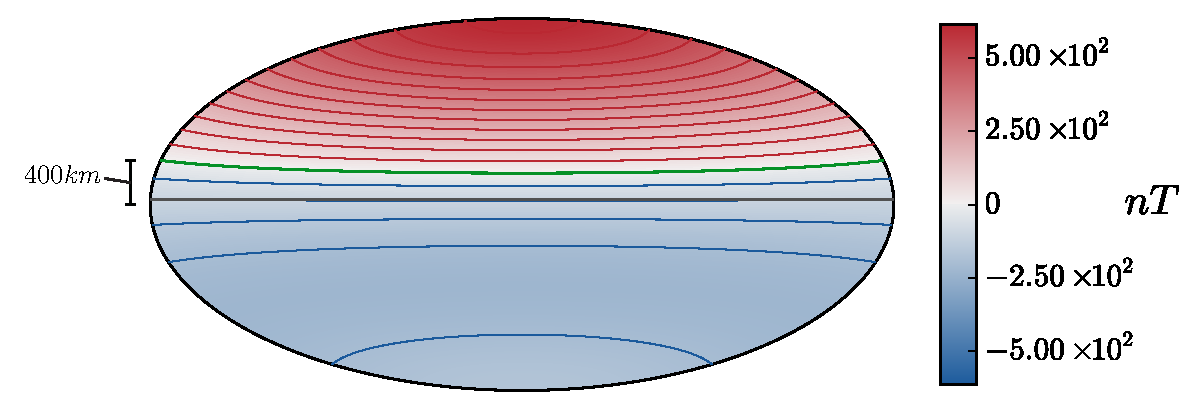
\includegraphics[width=\linewidth]{Chapter4/figures/Mercury_br.pdf}
	\caption{The surface radial magnetic field for all known Gauss coefficients ($\mathrm{g}_1^0$ and $\mathrm{g}_2^0$). The green horizontal line denotes the magnetic equator while the grey horizontal line denotes the planetary equator.}
	\label{fig:Mercurybr}
\end{figure}

\subsection{Dynamo Explanations for Mercury's Field}
One way a dynamo could produce a weak surface field is through a non-Earth-like field partitioning. There are several methods through which the magnetic field strength of Mercury can be estimated. One method assumes that to first order, the Coriolis and Lorentz forces will balance in the core; this is known as magnetostrophic balance (see section \ref{subsec:magnetostrophic}). Magnetostrophic balance implies an estimated magnetic field strength of $B=\sqrt{2\Omega\eta\rho\mu_{o}}$ where $\Omega$ is the rotation rate of the planet, $\eta$ is the magnetic diffusivity, $\rho$ is the density, and $\mu_o$ is the magnetic permeability of free space. If reasonable values are used for this estimate (Table \ref{tab:runs}), then a magnetic field strength within the core of $10^{5}-10^{7}$nT is obtained.

This estimation alone does not necessarily conflict with the observations of Mercury's field, since it predicts the magnetic field within the core while observations are made by spacecraft in the potential region outside the planet. The total magnetic field can be decomposed into poloidal $(\mathbf{B}_{P})$ and toroidal $(\mathbf{B}_{T})$ field components with the toroidal-poloidal  decomposition (see section \ref{sec:representations}):
\begin{equation}
\mathbf{B}=\mathbf{B}_{T}+\mathbf{B}_{P}=\nabla\times\left(T\hat{r}\right)+\nabla\times\nabla\times\left(P\hat{r}\right)
\end{equation}
where $T$ and $P$ are the toroidal and poloidal scalars, and $\hat{r}$ is the unit vector in the radial direction. Only the poloidal field has a radial component, and is therefore the only component that is observable from outside the core. If the Mercurian dynamo is similar to the Earth's in character, then there should be a similar partitioning between toroidal and poloidal field components. If the dipole moment at the core mantle boundary (CMB) is taken to be representative of the poloidal component, then it can be shown that for Mercury, $B_{dip}/B_{T}\approx10^{-2}-10^{-4}$, whereas for Earth $B_{dip}/B_{T} \approx 10^{-1}$  \citep{stevenson87}. The conclusion from this analysis is that if Mercury exists in the strong field regime (i.e. that the dynamo is in magnetostrophic balance), then a distinctly non-Earth-like field partitioning should be expected. Although this analysis is rather simplistic, it can be repeated using thermodynamic arguments instead of force balance arguments \citep{schubertandross88,stevenson87} resulting in similar total field strengths.

Several studies \citep{stanleyandbloxham2005,heimpelandaurnou2005,christensen06,takahashi06} have produced dynamo models with dipole moments of the same order as the observed Mercurian field through exotic field partitioning. This is accomplished either by making the inner core boundary (ICB) to core mantle boundary (CMB) radii ratios ($r_{io}$) very small ($0.15$ in \citet{heimpelandaurnou2005} or very large ($0.8$ in \citet{stanleyandbloxham2005}).

Another possibility is that Mercury's dynamo is not dipole dominated. Different scalings by \citet{OlsonandChristensen2006} have found that the dynamo should be in a state which produces a strong, multipolar dynamo. \citet{christensen06} used evidence that the temperature gradient across the core mantle boundary may be subadiabatic to justify a stably stratified layer occupying the top portion of Mercury's core. He argues from local Rossby number considerations (see section \ref{sec:rol}) that Mercury's dynamo should be multipolar, and that the surrounding stable shell preferentially attenuates higher multipoles, leaving a slowly varying, weak dipolar field. A subsequent study by \citet{manglik2010} showed that a growing inner core would release enough light element to disrupt any thermal stable stratification. They found this would lead to a strong, non-dipolar magnetic field. This means that a mechanism besides a subadiabatic heat flux is required to maintain the stable stratification if this mechanism is to work.

The final way that a weak surface field has been produced involves appealing to interactions with the solar wind. \citet{glassmaier2007} showed that Chapman-Ferraro currents induced by the interaction of Mercury's magnetosphere with the solar wind could produce magnetic fields in its core which  weaken the dynamo. Using a kinematic model based on work by \citet{levy1979}, they showed that this ``feedback dynamo'' could account for the weak observed magnetic field of Mercury. The initial temporal evolution of this model was further investigated by \citet{heyner2010} and it was modelled in a full, nonlinear dynamo model by \citet{heyner2011}.

All of these studies were done before the $g_2^0$ Gauss coefficient was measured by MESSENGER and none of them predicted $g_2^0$ accurately. Since the $g_2^0$ was measured, \citet{cao2014} published a study that used volumetric buoyancy and inhomogeneous heat flux thermal boundary conditions to shift the magnetic equator, however this study did not reproduce Mercury's weak observed magnetic field.

Because no model simultaneously reproduces both the weak field strength, and the equatorial displacement of the magnetic field (i.e. the correct $g_2^0$) we can conclude that the cause of Mercury's magnetic field remains an open question in planetary science.

\subsection{The State of Mercury's Core}

All dynamo explanations require that the core of Mercury remain at least partially liquid to the present day, something that is quite difficult to do with a small planet composed purely of iron. The detection of a dipolar magnetic field by Mariner 10 implied the existence of a liquid region due to the dynamo hypothesis, and observational evidence of longitudinal librations \citep{margot2007, margot2012} strongly suggests the existence of a liquid layer in Mercury. 

Although there is likely a liquid region in Mercury's core, the size of the liquid outer core is not well constrained. Most studies attribute the existence of a liquid outer core to the presence of a light element, such as sulfur, which would depress the freezing point of iron. Like the size of the inner core, the sulfur content of the outer core is not well constrained. Thermal evolution models \citep{schubertandross88} have shown that while it is difficult to prevent the core of a planet as small as Mercury from freezing, if the core contains some sulfur it is possible to keep the core partially liquid to the present day. If other effects such as temperature- and pressure-dependant rheologies \citep{conzelmann99,hauck04,brueur07} or tidal dissipation \citep{schubertandross88} are accounted for, almost any inner core to outer core radius ratio can be produced. As a result, the size of the inner core remains rather unconstrained. 

A recent study \citet{dumberry2015} used the moment of inertia and librational amplitude to extract further information about the state of Mercury's core. They find that the largest inner core compatible with these observations at the $1\sigma$ level is $1325 \pm 250\textrm{km}$ or $r_{io}=0.6\pm 0.1$.

Work by \citet{chenetal2008} has shown through a combination of new experiments on the non-ideal behavior of iron sulfur alloys at moderate pressures and existing data for higher-pressure melting of these alloys \citep{stewart07}, that Mercury may have a very different core crystallization regime than any other body, save possibly Ganymede \citep{hauck06}. The result is the formation of an iron precipitate at different radii throughout the core, the exact location and number of which is dependent on sulfur content. Once an iron precipitate forms, it begins to sink, while the residual, more sulfur-rich liquid rises. The generation of iron ``snow'' acts as a source of compositional convection, affecting fluid motions and therefore the dynamo.

If the liquid portion of the core contains between approximately 7 wt\% and 8 wt\% sulfur, an iron precipitate forms near the CMB and falls towards the inner core, this is referred to as a shallow snow state. For states with between approximately 8 wt\% and 10 wt\% sulfur, a snow layer at approximately 23 GPa and deeper will form as well (a double snow state). In this case we would expect two sources of compositional convection, one from the dense iron precipitate falling towards the planetary center, and another from the liberated sulfur floating towards the CMB. A schematic of the ``double snow state'' scenario is shown in figure \ref{fig:setup}(a). Finally, if the liquid outer core contains more than 10 wt\% sulfur, the snow zone at the CMB disappears, and only the deeper snow zone remains (a deep snow state). Although other light elements (such as O, Si, C, N, or H) can depress the freezing point of liquid iron, and could be present in Mercury's core, the iron-sulfur system is the best characterised. At this point there is no evidence to suggest snow zones occur in systems with different constituents. 

Here we use a numerical dynamo model to examine whether the effects of snow zones on Mercury's dynamo could explain its weak magnetic field. In the following sections we discuss a method of incorporating snow zones into the models, and the characteristics of the resulting fields. In this study we focus on double and deep snow states, since previous work demonstrated that shallow snow state models produce Earth-like dipole intensities when in magnetostrophic balance \citep{stanleyandmohammadi}.

We also exclude double and deep snow states in which the deep snow zone extends all the way to the ICB. In this scenario, motions in the lower region of the dynamo would be very small scale, since this region would be in a diffusive staircase convection regime. A state similar to this has already been explored by \citet{stanleyandbloxham2006} in the context of Uranus and Neptune. They found that strong, multipolar fields result, which do not match the observed field of Mercury.

\section{Modelling a Snow Zone}
To model a snow zone in a numerical dynamo model, we first observe that as iron solidifies it injects buoyancy into the core. For example, in Earth pure iron solidifies at the inner core boundary and the residual light element is released into the fluid. This light element is now lighter than the bulk fluid and is therefore buoyant. We can use similar reasoning to add a snow zone to a numerical dynamo model. There are two effects which need to be taken into account when implementing a snow zone. First, the negative buoyancy representing the sinking iron, and secondly the positive buoyancy due to the remaining sulfur rich fluid.

To incorporate both effects, we model a single snow zone as two thin shells: a source of co-density directly above a sink of co-density. The background co-density profile $C_{0}\left(r\right)$ is then determined by solving equation (\ref{eq:dimensionalbgcodensity}) with the given $Q\left(r\right)$. We find that a snow layer can be represented as a stably stratified layer in the slope of the background co-density profile. For the sake of simplicity, we make it a layer of constant $d C_{0}\left(r\right)/dr$ (figure \ref{fig:setup}(b)). It should be noted that this representation of a snow layer does not attempt to capture the specific dynamics of iron snow, but rather their net effects. Our model of a snow layer is quite crude, it will be the goal of future studies to make it more realistic.
\begin{figure}
	\centering
	\noindent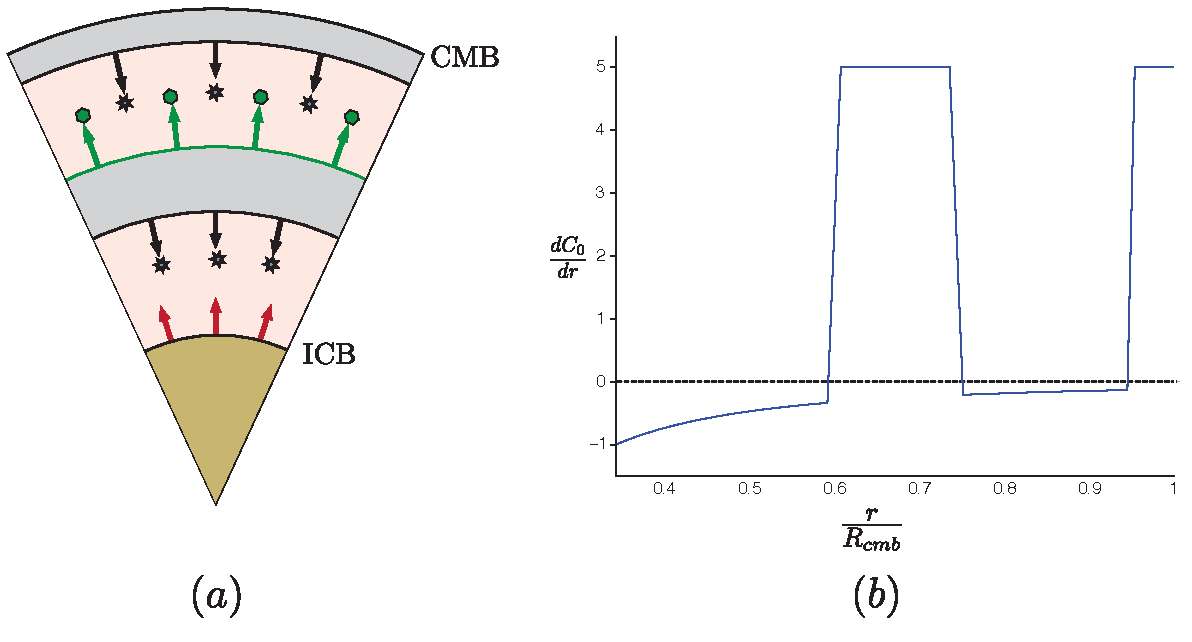
\includegraphics[width=40pc]{Chapter4/figures/setup.pdf}
	\caption{a) A schematic diagram of a core in a double snow state, the snow layers are indicated by the grey bands. The compositional effects are indicated by arrows, sulfur driven effects are indicated in green hexagons, while iron driven effects are in black stars, thermally driven effects are indicated by red arrows. b) The slope of the background co-density profile for a double snow state. Areas of positive $dC_{0}/dr$ indicate stably stratified regions, or snow zones. The dashed line indicates the neutral buoyancy profile ($dC_{0}/dr=0$).}
	\label{fig:setup}
\end{figure}

Our representation of a snow layer as a stably stratified region makes physical sense if we consider the path of an individual parcel buoyant at the ICB. This parcel will begin to rise, and will remain buoyant and rise until it reaches the base of the deep snow layer where it begins to solidify, expelling any light element mixed in with it, and losing its buoyancy. It then descends back into the lower layer. In this regard, the base of the snow layer is both a stably stratified layer (reducing the buoyancy of the rising parcel) and a source of compositional buoyancy in the lower layer (releasing iron which is denser than its surroundings). Similarly, the sulfur released in the deep snow layer is more buoyant than the fluid immediately above the deep snow layer and acts as a source of buoyancy for the upper region. For simplicity we do not consider the energy associated with latent heat release and consumption. Since compositionally driven convection is thermodynamically more efficient than the thermal component of convection, this is likely a reasonable first-order assumption.

As a result of the large uncertainties associated with many of the quantities in planetary cores, the strength of the stable stratification due to the snow layer is unknown. In our models, we assume that the compositional sources of buoyancy resulting from iron snow zones are the primary driver of convection within Mercury, thus the stably stratified layer would be strongly stratified relative to the co-density flux at the inner core boundary. We found that our results remained largely the same so long as the snow layers are the primary driver of convection in our models.

The thickness of the snow layer is another quantity which can vary widely depending on the sulfur content and on the adiabat \citep{chenetal2008}. We have chosen a deep snow layer thickness of $0.13 r_{o}$. This falls within the range of values predicted from the data in \citet{chenetal2008}. Investigating the effect of snow layer thickness on the dynamo will be the goal of future work in this field. In this study, the deep snow zone extends from $0.61 R_{CMB}$ to $0.74 R_{CMB}$, where $R_{CMB}$ is assumed to be $0.75 R_{M}$.

In all cases the maximum spherical harmonic degree is 33 and the maximum order is 21. In the radial direction we used 119 grid points, 36 of which were in the inner core, 64 of which were in the fluid region and 19 of which were in the thin, weakly conducting mantle layer.

The models presented here used hyperdiffusivities (equations \ref{eq:hyperdiffseta}-\ref{eq:hyperdiffsnu}) with $\hat{\eta}=\hat{\kappa}=0.06$ and $\hat{\nu}=0.05$. Preliminary results on higher resolution runs ($L_{max}=90$, $m_{max}=85$, $n_{r}=95$) show that the resolution we run our models at is not an issue when hyperdiffusivities are used ($l_{o}=0$).

In all models presented here, constant co-density flux boundary conditions were applied to both the inner core boundary and the core mantle boundary. When constant co-density boundary conditions were used instead, there was no significant qualitative differences in the models. 

In all cases we kept the inner core to outer core radius ratio ($r_{io}$) fixed at $12/35$. This is consistent with the predictions of \citet{hauck04} when they used sulfur contents high enough to develop double and deep snow states. In our study we chose a moderately low Ekman number of $2\times10^{-5}$ to reduce the effects of viscosity in our model. Although this is much larger than the Ekman number expected for Mercury (on the order of $10^{-13}$), at present it is numerically infeasible to work at such low Ekman numbers. Stress free boundary conditions are also used to minimise Ekman boundary layer effects, which would be far too large if we chose to use no-slip boundary conditions. We used finite electrically conducting boundary conditions on the magnetic field. We also set our magnetic Rossby number to be $2\times10^{-5}$, and set both of our Prandtl numbers to 1. Only the modified Rayleigh number  and initial conditions were varied between the models. In these models the critical Rayleigh number is approximately $700$.

\section{Results}
\subsection{Dipole Moment}

\citet{chenetal2008} outline three basic configurations for iron snow zones in Mercury's core: a single snow zone at the CMB (shallow snow state), a snow zone at the CMB along with one midway through the core (double snow state), and a single snow zone midway through the core (deep snow state). We found that only models with a deep snow layer (double and deep snow states)  which does not extend to the ICB successfully produced a weak dipolar field.  The results for the simulations of interest are summarised in Table \ref{tab:runs}. In all cases the dipole moment was relatively stable. Although several dipole reversals did occur, the field usually returned to a stable configuration akin to its pre-reversal state, though of opposite polarity. In most models the dipole tilt is quite small, for a non-reversing segment of model 2, the dipole tilt averaged over approximately half a magnetic diffusion time was $6^{\circ}$ away from the rotation axis.
\begin{table*}
\centering
%\begin{tabular}{c c  l  r @{.} l   r @{.} l   r @{.} l   r @{.} l   r @{.} l   r @{.} l   r @{.} l r @{.} l r @{.} l  }
%Model & Ra & Model Type & \multicolumn{6}{c}{Dipole Moment} & \multicolumn{6}{c}{$B_{dip}/B_{T}\times10^{-3}$} & \multicolumn{4}{c}{L (Normalized)} \\
%   &                     & &  \multicolumn{2}{c}{Mean} & \multicolumn{2}{c}{Max}   & \multicolumn{2}{c}{Min} & \multicolumn{2}{c}{Mean} & \multicolumn{2}{c}{Max} & \multicolumn{2}{c}{Min} &    \multicolumn{2}{c}{2} &  \multicolumn{2}{c}{3}  \\
 %  \hline
%1 & 50000 &  Double Snow State & 174&1 & 278&2 & 75&6 &  4&06 &  30&3 & 0&42 & 0&069 & 0&37 \\ %subrun 43 2300 2750
%2 & 55000  & 202&1 & 278&1 & 132&0 & 2&85 &  12&1 & 0&66 & 1&0 & 0&069 & 0&37 & 0&036 & 0&058 \\ %subrun 44 2300-2600
%2 & 55000 & Double Snow State & 152&1 & 224&7 & 57&9 & 2&07 & 8&2 & 0&61 & 0&097 & 0&15 \\ %21.031 1200-1400
%3 & 50000 & Double Snow State &  360&1& 616&6 & 137&7 & 2&50 & 10&9 & 0&44 & 0&091 & 0&24 \\ %subrun 36 1200-1547
%4 & 55000 & Single Snow State & 939&1& 1421&0 & 660&8& 4&64 & 11&7 & 1&55 & 0&0096 & 0&085  \\% 21.027 1200-2228
%5 & 30000 & Single Snow State & 1388&5 & 1477&0 & 1281&0 & 9&02 & 12&7 & 4&56 & 0&0012 & 0&011 \\%19.032 1700-2000
 %Add some other core size
%\end{tabular}
%!TEX root = ../../thesis.tex
\begin{tabular}{cccrrrllrrlll}
\multicolumn{3}{l}{}                                               & \multicolumn{3}{c}{Dipole Moment}                                            &  & \multicolumn{3}{c}{$B_{dip}/B_{T}\times10^{-3}$}                             &  & \multicolumn{2}{c}{Normalized}                               \\
\multicolumn{1}{l}{} & \multicolumn{1}{l}{} & \multicolumn{1}{l}{} & \multicolumn{3}{c}{$nT-Rm^3$}                                                &  & \multicolumn{3}{l}{}                                                         &  & \multicolumn{2}{c}{Power (deg)}                              \\  \cline{4-6} \cline{8-10} \cline{12-13} \\[-1.5ex]
Model                & Ra                   & Model Type           & \multicolumn{1}{c}{Mean} & \multicolumn{1}{c}{Max} & \multicolumn{1}{c}{Min} &  & \multicolumn{1}{c}{Mean} & \multicolumn{1}{c}{Max} & \multicolumn{1}{c}{Min} &  & $P_2/P_1$   & \multicolumn{1}{c}{$P_3/P_1$} \\ [.8ex]\hline
1                    & 50000                & Double Snow          & 190                      & 304                     & 82                      &  & 4.06                     & 30.3                    & 0.42                    &  & 0.069       & 0.37                                           \\
2                    & 50000                & Double Snow          & 394                      & 676                     & 151                     &  & 2.50                     & 10.9                    & 0.44                    &  & 0.091       & 0.24                                           \\
3                    & 55000                & Double Snow          & 166                      & 246                     & 64                      &  & 2.07                     & 8.2                     & 0.61                    &  & 0.097       & 0.15                                           \\
4                    & 30000                & Deep Snow            & 1520                     & 1617                    & 1403                    &  & 9.02                     & 12.7                    & 4.56                    &  & 0.0012      & 0.011                                           \\
5                    & 55000                & Deep Snow            & 1028                     & 1556                    & 724                     &  & 4.64                     & 11.7                    & 1.55                    &  & 0.0096      & 0.085                   
\end{tabular}
\caption{{\bf Parameter values and field strength results:}  In this table, runs that have the same Rayleigh number have different initial conditions. We did this to ensure that the observed ``double dynamo'' state is robust. $P_{L}$ refers to the power in the $L$th degree of the spherical harmonic power spectrum at the surface. The redimensionalization and field strength estimates use $\Omega=1.24\times10^{-6} \mathrm{s}^{-1}$, $\rho=7200$ $\mathrm{kg}$/$\mathrm{m}^3$ (which is the same as is used in \citep{hauck04}, $\mu_{0}=4\pi\times10^{-7} \mathrm{m} \mathrm{kg}/\mathrm{s}^{2}\mathrm{A}^{2}$, $U\approx 10^{-3} \mathrm{m}/\mathrm{s}$, $L\approx 1800\mathrm{km}$, and $\eta=2\mathrm{m}^{2}$/$\mathrm{s}$. Of these, the length scale and the velocity estimation are the least certain.}
\label{tab:runs}
\end{table*}

\subsection{Velocity Fields}
The most immediate effect of the deep snow layer is to isolate the regions above and below the layer, there is very little fluid flowing across the snow layer. Convection columns form in both convecting regions, and do not appear to have any spatial or temporal correlation. In figure \ref{fig:vorticity}
\begin{figure}
	\centering
	\noindent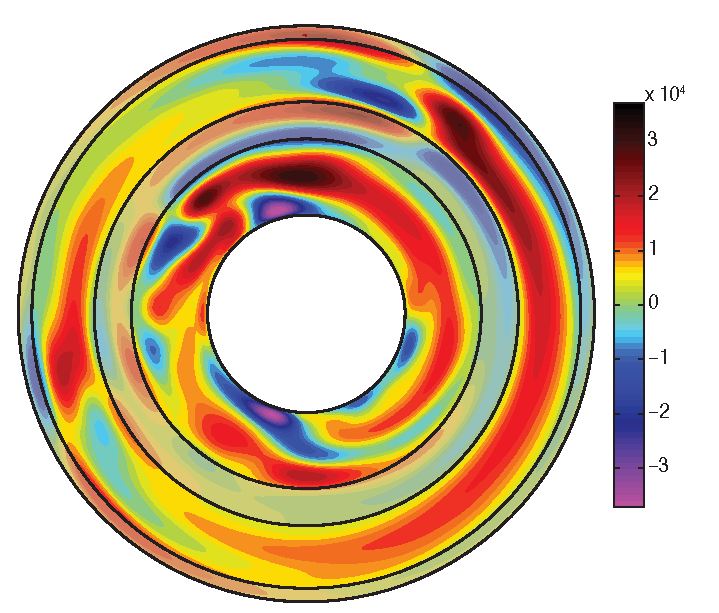
\includegraphics[width=.6\linewidth]{Chapter4/figures/wz19_043_2500_00.pdf}
	\caption{A snapshot of axial vorticity in the equatorial plane for a double snow state model (model 1). Here, the snow layers have been shaded grey. The units in this figure are non-dimensional.}
	\label{fig:vorticity}
\end{figure}
the axial vorticity in the equatorial plane is plotted. The regions of solid colour correspond to convection columns aligned with the rotation axis and the sign of the vorticity indicates the direction the column is rotating. The convection columns are coaxial with the rotation axis and do not cut across the stably stratified layer. Although there are patches of vorticity inside the stable layer, these are all due to viscous coupling to an opposite patch of vorticity in the convective region and do not contribute to dynamo generation processes.

The snow layer also has consequences for the axisymmetric flows. In figure \ref{fig:uax}
\begin{figure}
	\centering
	\noindent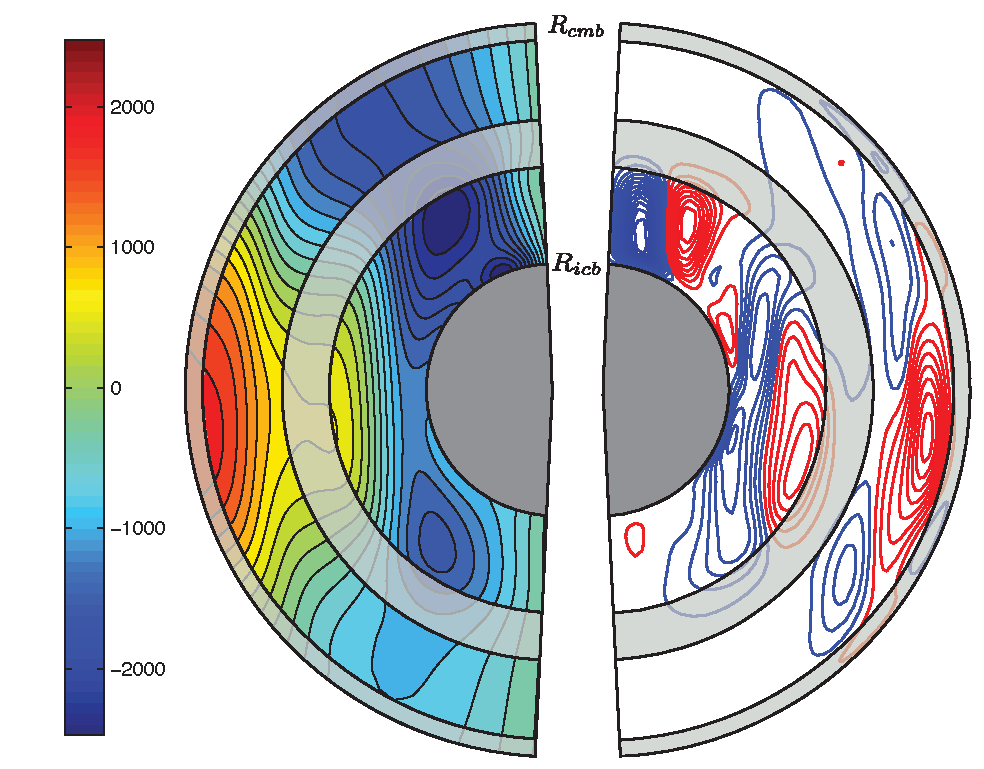
\includegraphics[width=.6\linewidth]{Chapter4/figures/uxtpavg19_043_2460-2530}
	\caption{Contours of the axisymmetric toroidal component of the velocity (left) and streamlines of the axisymmetric poloidal velocity (right) for a double snow state model, averaged over $0.35$ dipole magnetic diffusion times. In the right plot the colour denotes the direction of the flow, red is clockwise and blue is counterclockwise. Here, the snow layers have been shaded grey. The units in this figure are non-dimensional.}
	\label{fig:uax}
\end{figure}
 the axisymmetric toroidal (left) and poloidal (right) components of velocity are plotted. Examining the toroidal component of velocity, we see that the snow zones, especially the deep snow zone, bend the zonal flow contours significantly. The regions closest to the rotation axis are dominated by a retrograde flow, while the regions in the equatorial region near the CMB have an overall prograde flow. Examining the poloidal velocity field (figure \ref{fig:uax} (right)) we see that most of the poloidal flow occurs in the inner dynamo region. In the outer region, convection is concentrated in the equatorial region with little convection occurring inside the tangent cylinder formed by the deep snow layer. 

\subsection{Magnetic Field}
The nature of this dynamo is revealed if we examine the generation mechanisms for both toroidal and poloidal fields. Figure \ref{fig:maggen} (a) shows the axisymmetric toroidal field for a double snow state model.
%
\begin{figure}
	\centering
	\noindent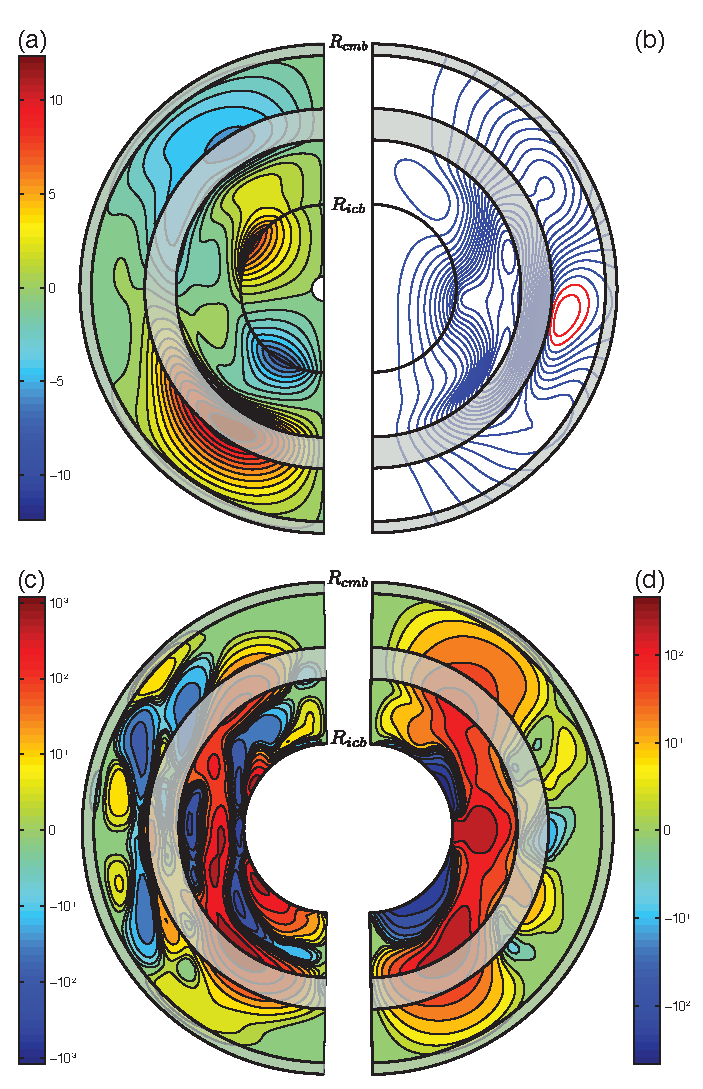
\includegraphics[width=.7\linewidth]{Chapter4/figures/aximaggen}
	\caption{(a) Contours of the axisymmetric component of the toroidal field for a double snow state model. (b) Streamlines of the axisymmetric poloidal field for a double snow state model. The colour of the streamline denotes the direction of the field, red is clockwise and blue is counterclockwise. (c) An axisymmetric slice of the generation of toroidal magnetic field energy due to stretching of poloidal magnetic field ($\overline{\mathbf{B}_{T}\cdot\left[\left(\mathbf{B}_{P}\cdot\nabla\right)\mathbf{u}\right]}$) for a double snow state model. (d) An axisymmetric slice of the generation of poloidal magnetic field energy due to stretching of toroidal magnetic field ($\overline{\mathbf{B}_{P}\cdot\left[\left(\mathbf{B}_{T}\cdot\nabla\right)\mathbf{u}\right]}$) for a double snow state model. All the plots in this figure are from model 1, and have been averaged over the same period as figure \ref{fig:uax}. The snow layers have been shaded grey. The units in this figure are non-dimensional.}
	\label{fig:maggen}
\end{figure}
%
When compared to an Earth-like model (i.e. no snow zones) (figure \ref{fig:toroidalpoloidalearth}, left), it appears as though there are two dynamos of opposite polarity operating within the same core of the double snow state model.
%
\begin{figure}
	\centering
	\noindent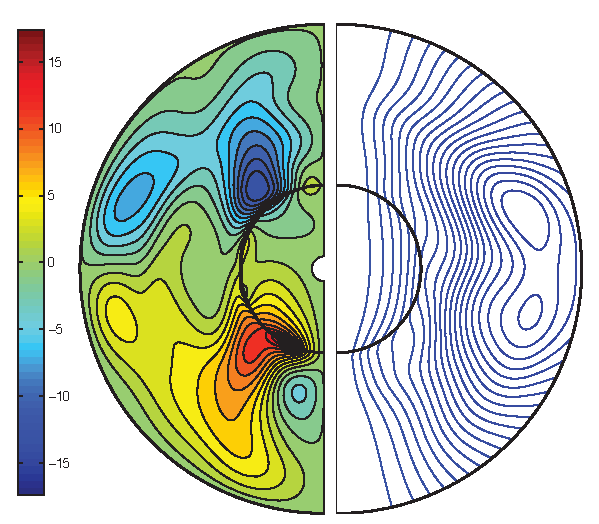
\includegraphics[width=.6\linewidth]{Chapter4/figures/BTorPolEarth}
	\caption{Contours of the axisymmetric component of the toroidal field (left) and streamlines of the axisymmetric poloidal field (right) for a snapshot of a strong field, Earth-like model (i.e. a model with no snow zones).  The units in this figure are non-dimensional.}
	\label{fig:toroidalpoloidalearth}
\end{figure}
%
Further evidence for this ``double dynamo'' interpretation is found by examining the radial magnetic field at the CMB (figure \ref{fig:brad}, top).
\begin{figure}
	\centering
	\noindent\includegraphics[width=\linewidth]{Chapter4/figures/Brad_dim.pdf}
	\caption{The radial magnetic field for model 1 at the CMB (top) and at  the surface (bottom) at the same instant in time as figure \ref{fig:vorticity}. The tangent cylinder formed by the deep snow layer has been shaded grey. }
	\label{fig:brad}
\end{figure}
In figure \ref{fig:brad} the intersection of the tangent cylinder formed by the deep snow zone with the CMB is shaded grey. We note that there seem to be no features in the radial magnetic field at the CMB from the tangent cylinder of the inner core \citep{stanleyfluxspot}, while the deep snow zone's tangent cylinder serves as the border between radial field of opposing sign. Also, the prominent flux spots in the equatorial region do not occur poleward of the tangent cylinder formed by the deep snow layer.

In figure \ref{fig:brad} (top), which plots the radial component of the magnetic field at the CMB for model 1, a strong octupolar signature is seen (figure \ref{fig:power}, Table \ref{tab:runs}).
\begin{figure}
	\centering
	\noindent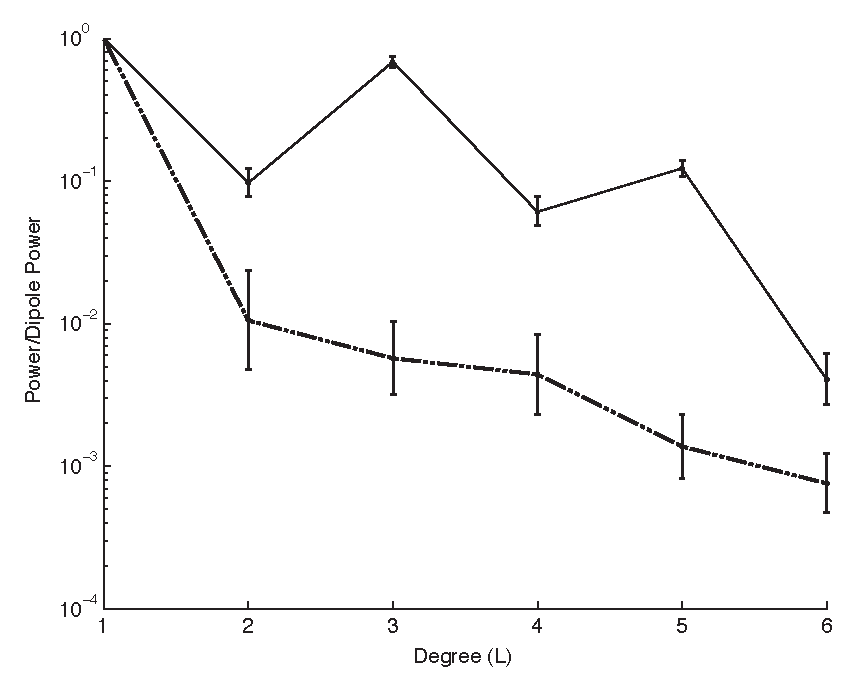
\includegraphics[width=30pc]{Chapter4/figures/powermodel.pdf}
	\caption{Temporally averaged surface power spectra for an Earth-like model (i.e. a model without snow zones) (dashed) and for a double snow state model (solid, model 1) averaged over the same time period as figure \ref{fig:uax} at the surface of a Mercury-like planet ($R_{\mathrm{cmb}}=0.75$). Both models have been averaged over $0.35$ dipole magnetic diffusion times. The error bars on the power spectrum for the model indicate one standard deviation of the power over the averaging window.}
	\label{fig:power}
\end{figure}
The magnetic field generated by the dynamo region nearest to the inner core is expressed in the polar regions, while the equatorial regions are dominated by the field generated in the outer dynamo region. If we observe the radial magnetic field for different radii inside the core,  the inverted polarity in the equatorial region does not appear until outside the deep snow zone, indicating a source in the outer dynamo region.

While the dipole moment of these dynamo models matches the dipole moment of Mercury quite well, the model $\mathrm{g}_2^0$ Gauss coefficient is not matched as well. In figure \ref{fig:gauss} we plot $\mathrm{g}_2^{0}$ against $\mathrm{g}_1^{0}$ at each timestep output by all of our double snow state models. The observations from the MESSENGER mission of $\mathrm{g}_1^{0}$, and $\mathrm{g}_2^{0}$ are shown as grey rectangles, with the size of the rectangles denoting the uncertainty associated with the measurements. In this figure there are two areas that match Mercury's magnetic field, this is due to the north-south symmetry present in the magnetic induction equation. The important value to match is the magnitudes and relative signs of these two Gauss coefficients. In figure \ref{fig:gauss} we see that model 1 briefly matches Mercury's magnetic field, however most of the time the $\mathrm{g}_2^0$ field component is too small or has the wrong sign to be compatible with the MESSENGER measurements. 
\begin{figure}
	\centering
	\noindent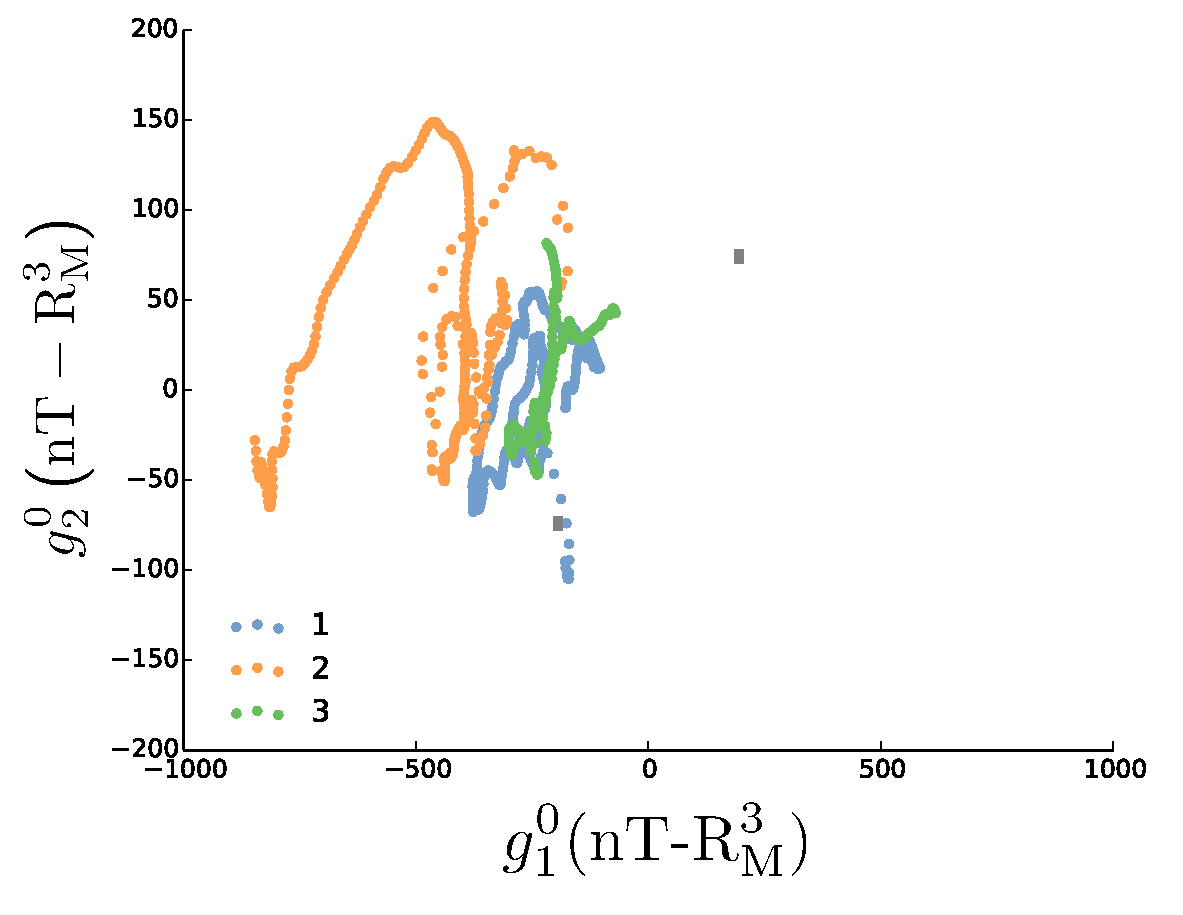
\includegraphics[width=30pc]{Chapter4/figures/g10g20.pdf}
	\caption{The axial dipole and quadrupole Gauss coefficients for the double snow state models in this study. The grey boxes denote areas of the plot which would match the MESSENGER observations of Mercury's magnetic field to within uncertainties. Here the numbers in the legend refer to the run numbers in Table \ref{tab:runs}.}
	\label{fig:gauss}
\end{figure}

\subsection{Dynamo Mechanism}
\subsubsection{Generation of the Toroidal Field}
The inverted polarity of the toroidal magnetic field in the outer region can be understood by examining the dominant $\omega$-effect component of the toroidal field generation in our models. From equation (\ref{eq:nondimmagnetic}), the growth of axisymmetric energy in the toroidal magnetic field can be written as
\begin{equation}
\mathbf{B}_{T}\cdot\frac{\partial \mathbf{B}_{T}}{\partial t}=\mathbf{B}_{T}\cdot\left[\left(\mathbf{B}\cdot\nabla\right)\mathbf{u}\right]-\mathbf{B}_{T}\cdot\left[\left(\mathbf{u}\cdot\nabla\right)\mathbf{B}\right].
\end{equation}
The first term on the right describes the growth of energy in the toroidal field due to stretching of magnetic field lines while the second describes the growth of toroidal field energy due to the advection of toroidal field. Focussing on the stretching term, the direction of the resultant toroidal field is dependent on the direction of the initial field and on the sign of the gradient of velocity which is shearing it. Figure \ref{fig:uax} (left) shows the axisymmetric toroidal component of the flow. Here, the stably stratified layer causes differential rotation in the $z$ direction. Examining the midlatitude regions where the flow is strongest, we see that the gradient in $\mathbf{u}$ changes sign just below the stable layer. An initially poloidal magnetic field which originates from the inner dynamo will be sheared by this differential rotation. The shear in the outer region will generate toroidal field which is opposite in sign to the toroidal field in the inner region. This process can be seen in figure \ref{fig:maggen} (c), which plots the axisymmetric growth of toroidal field energy caused by the stretching of poloidal magnetic field lines ($\overline{\mathbf{B}_{T}\cdot\left(\mathbf{B}_{P}\cdot\nabla\right)\mathbf{u}}$). We see that significant amounts of poloidal field are converted into toroidal field in the mid-latitudes of the outer region and deep snow layer, effectively seeding the outer region with toroidal field. Although there are other ways that toroidal field can be generated in the outer region (for example by stretching toroidal field) this is the dominant method in our models. Figure \ref{fig:schematictoroidal} shows a schematic diagram of this process.
\begin{figure}
	\centering
	\noindent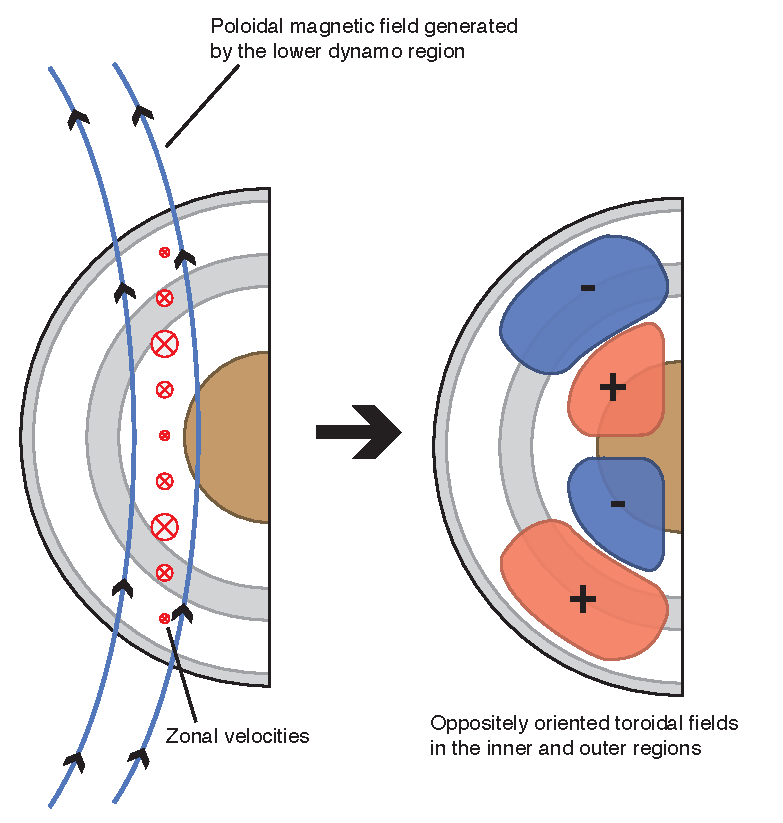
\includegraphics[width=30pc]{Chapter4/figures/Schematic-Toroidal.pdf}
	\caption{A schematic diagram of the generation of the toroidal field in a double snow state model. On the left, red arrowheads (going into the page) represent zonal velocities whose strength is proportional to the arrow head size. Moving in the direction of the poloidal field line, an increase in zonal velocity (i.e. a positive gradient) results in  positively signed toroidal field generation. Conversely, a decrease in zonal velocity (i.e. a negative gradient) results in negatively signed toroidal field generation. These act on poloidal magnetic fields (blue) to create the characteristic toroidal field we observed in our models. The snow layers have been shaded grey.}
	\label{fig:schematictoroidal}
\end{figure}

\subsubsection{Generation of the Poloidal Field}
Poloidal fields in both the inner and outer regions are generated by convective motions acting on toroidal fields. In the inner region, convection is stronger and a strong dipolar field is generated. However, the dipole field observed outside the core is weak due to a combination of three processes, which all stem from the presence of a deep snow layer. A schematic diagram illustrating these three processes is shown in figure \ref{fig:schematicpoloidal}.
\begin{figure}
	\centering
	\noindent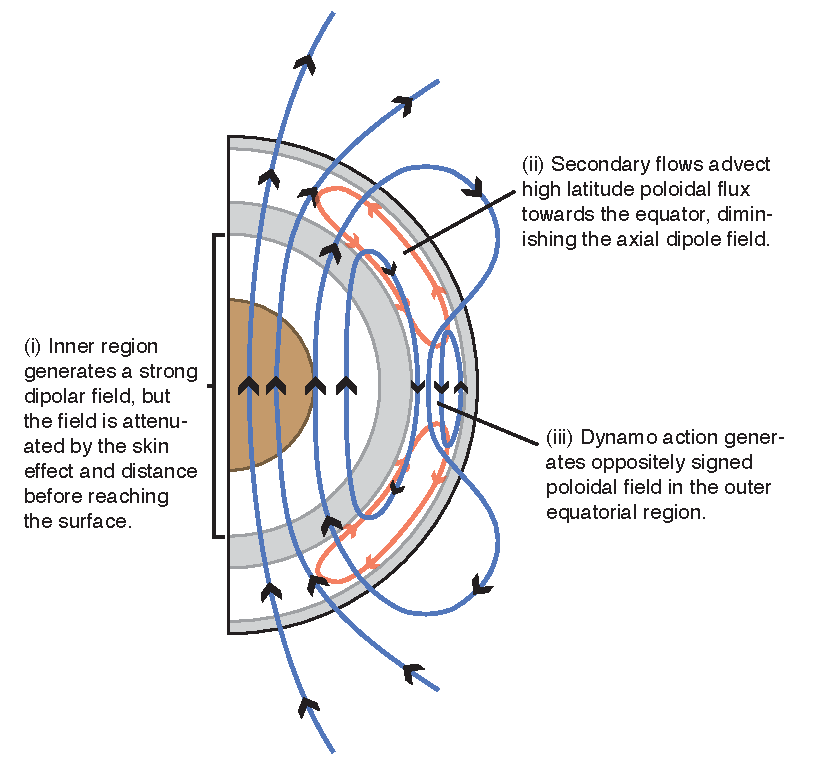
\includegraphics[width=30pc]{Chapter4/figures/Schematic-Poloidal.pdf}
	\caption{A schematic diagram of the generation of the poloidal magnetic field in a double snow state model. In this figure blue lines represent poloidal magnetic field lines, and red lines represent meridional flows. The three mechanisms discussed in the text for weakening the observed field are marked (i), (ii), and (iii). The snow layers have been shaded grey.}
	\label{fig:schematicpoloidal}
\end{figure}

First, the inner dynamo region does most of the field generation, but since it is removed from the CMB (due to the presence of the outer layer), its strength is reduced. This is similar to the mechanism behind the weak magnetic field observed in \citet{christensen06} however, this is not the sole reason for the overall weakness of the field in our models. In  \citet{christensen06} the parameters were chosen such that magnetic field at the top of the dynamo generation region was both strong and non-dipolar. Although placing the dynamo generation away from the surface does weaken the dipole moment observed at the surface, the primary reason their model possesses a weak dipole moment is because most of the power lies in higher multipoles which vary quickly in time and are preferentially attenuated due to the skin effect. To determine whether our fields are weak solely due to the skin effect, we ran a deep snow state model, in which the region above the lower boundary of the deep snow zone was strongly stably stratified. This ensured that no dynamo action would occur in the outer region, and that any weakening of the field observed would be solely due to the skin effect or the removal of the dynamo region from the surface. We found that when we did this, the magnetic field was stronger than in our models containing a convective upper region by approximately an order of magnitude. From this analysis we conclude that flows in the outer region play an important role in the attenuation of the overall field in our models.

Secondly, additional weakening of the dipole moment in our models occurs through the theft of flux by meridional flows in the outer dynamo region. The density of poloidal magnetic field lines is reduced in the mid-latitudes of the outer region in figure \ref{fig:maggen} (b), as the field lines are advected towards the equator by meridional flows in this region (see figure \ref{fig:schematicpoloidal} for a schematic representation of this).

Finally, dynamo action in the outer region weakens the observed surface field. The conversion of the toroidal field in the mid-latitudes of the outer region into poloidal field can be seen when we plot the axisymmetric growth of poloidal field energy caused by the stretching of toroidal magnetic fields ($\overline{\mathbf{B}_{P}\cdot\left(\mathbf{B}_{T}\cdot\nabla\right)\mathbf{u}}$) which is plotted in figure \ref{fig:maggen} (d). When this is compared with the axisymmetric streamlines of poloidal magnetic field in figure \ref{fig:maggen} (b) we see that the source of the equatorial poloidal field we observe is the mid-latitude toroidal flux sheared out by the snow layer. Since the outer dynamo region is seeded with toroidal field which is opposite in polarity to that of the inner dynamo region, convection will generate a poloidal field in the outer region of opposite sign to the field generated by the inner region. Evidence that the outer dynamo region would operate in this way comes from studies of dynamos in thin shells (similar to the geometry of the outer shell) which show that at similar Rayleigh numbers to the ones used here, dipolar fields result \citep{stanleyandmohammadi}. In the outer region we observe a very similar field morphology as \citet{stanleyandmohammadi}, implying that if both regions generated poloidal field independently, the resulting fields would be of opposite polarity. Since they occur within the same core, they superpose and contribute to the weak observed surface field. 

The polarity of the outer dynamo is entirely determined by the inner dynamo. Since the outer region is being primed with a toroidal field by the inner region, and since convection is relatively weak in the outer region, it is unlikely that this dynamo could ever determine it's polarity independent of the inner region. The situation of a dynamo being immersed in an externally applied field was examined by \citet{sarson97}. In that case a dynamo was immersed in a constant background field, giving the dynamo an external source of poloidal field, which it could then convert to toroidal field. In our case the opposite occurs, the inner dynamo region supplies the outer dynamo region with a toroidal field which this region then converts to poloidal field. 

When a double snow state model reverses, it is the inner dynamo that leads the reversal. During the reversal, the dipole moment decays to only a few nT-$R_{M}^3$. After the reversal finishes, the same differential rotation in $z$ occurs, so the outer dynamo region once again becomes active with the opposite sign as the inner dynamo region. 

In our models we chose parameters such that the magnetic Reynolds numbers of our snow zone models are comparable to the Earth-like dynamo model in figure \ref{fig:toroidalpoloidalearth}. We define our magnetic Reynolds number as
\begin{equation}
\mathrm{Re}_{M}=\frac{1}{V}\int_{V}\frac{\left|\nabla\times\left(\mathbf{u}\times\mathbf{B}\right)\right|}{\left|\nabla^{2}\mathbf{B}\right|}.
\end{equation}
We have done this to ensure that any change in field strength we observe is not the result of a different efficiency of magnetic field generation. The difference in the field intensity at the surface can therefore be attributed to the change in field morphology resulting from the snow zones. Other studies  \citep{christensen06scaling} have shown that Earth-like dynamo models have a critical magnetic Reynolds number of order 50. The Earth-like dynamo model in figure \ref{fig:toroidalpoloidalearth} and our double snow state models have magnetic Reynolds numbers in the range of $48$-$62$.

\section{Discussion}
We have shown that introducing exotic (yet predicted) sources of compositional driving can produce a dipole moment as weak as the measured moment of Mercury. Although both the deep and double snow states produced dipole moments weaker than one would expect from scaling arguments, the double snow states most closely match the observations of Mercury. The deep snow state is also less likely than the double snow state due to the high ($>10\%$wt) sulfur content it requires \citep{rivoldini09}. The results of this work are published in \citet{vilim2010}.

Owing to the reduction in length scale caused by the addition of the stably stratified layer, our models in a double or deep snow state geometry must operate at Rayleigh numbers which are more than $40$ times supercritical in order to sustain a magnetic field against ohmic decay. For example, although they use a slightly different geometry and different boundary conditions, \citet{christensen06} show that $\mathrm{Ra}>50\mathrm{Ra}_{c}$ for dynamo onset in the parameter regime of our snow zone models (in order to make this comparison, one must convert our definition of the Ekman number to one in terms of shell thickness rather than core radius, using the thickness of the lower dynamo region as the shell thickness). Since we must operate at highly supercritical Rayleigh numbers, we must turn to hyperdiffusivities for computational reasons. We have run high resolution runs  ($L_{max}=90$, $m_{max}=85$, $n_{r}=65$) at lower ($7.9 Ra_{c}$) supercritical Rayleigh numbers with minimal ($l_{o}=40$, in equations (\ref{eq:hyperdiffseta})-(\ref{eq:hyperdiffsnu})) or absent hyperdiffusivities, however these supercriticalities are too low to sustain magnetic fields. The absence of dynamo action at these low Rayleigh numbers when hyperdiffusivites are not used implies that small scale fluid motions, which are preferentially damped in our models that use hyperdiffusivities, are not responsible for the large scale field generation.

The mechanisms behind the formation of the dynamo state we observe are expected to be robust to hyperdiffusivities. Fluid motions in the lower dynamo region should produce a dipolar seed field irrespective of whether hyperdiffusivities are present. The principle reason for the pattern of toroidal fields we observe in our study is differential rotation in the radial direction at mid-latitudes. Finally, the transport of flux towards the equator is caused by large scale secondary flows which occur in dynamos without hyperdiffusivies as well. 

This system is likely to evolve in time substantially. Over long timescales the upper dynamo region should become preferentially enriched in sulfur and the lower region should become preferentially enriched in iron and eventually stratified down to the ICB as the zone of potential snow formation grows with cooling. Furthermore, the region nearest the CMB could form a stratified layer of light element similar to the kind proposed for the Earth \citep{Braginsky2006}. This stratified ocean would co-exist with the stratified region which we have already placed near the CMB. All these effects vary on timescales much longer than those associated with the dynamo, so they have been neglected here. Future work will focus on understanding the long term thermal and compositional evolution of a double snow state system. However, should future observations of Mercury's magnetic field confirm field characteristics consistent with the double snow zone model, this would place important constraints on the present-day structure of the planet's core.

In this study we have only examined situations that result in the outer dynamo region generating little field on its own. Understanding the consequences of increasing the Rayleigh number, which should lead to an increase the vigor of convection in the outer dynamo region will be an area of interesting future research.

The magnetic field produced by a geometry containing a deep snow layer is quite distinct. For the $r_{io}$ value used in this study ($0.34$), the octupole component is always much larger than the quadrupole component and is comparable to the dipole component.

















